Несмотря на то, что программа уже работоспособна, есть ещё много идей и планов по её усовершенствованию:


 \subsection{Внедрить \textit{быстрый пересчёт функции ошибки}}
Это улучшение давно напрашивается,
но оно несколько теряет в эффективности из-за того, что в одной мутации в среднем изменяется
не так мало мазков (однако это количество убывает со временем).
В настоящий момент ведётся работа над внедрением.

\subsection{Разделение мазков по слоям}
 Нетрудно заметить, что при рисовании картин художники сначала проходятся по холсту черновыми мазками большого размера, а затем — прорабатывают детали.
 Таких уровней детализации зачастую бывает немало.

 Пример того, как художник (\url{https://www.youtube.com/watch?v=VaXHtai2alU}) рисует картину по слоям:

\begin{figure}[h!]
    \centering
    \subfloat{\includegraphics[width=0.24\textwidth]{painting_example_layer_0.png}}
    \subfloat{\includegraphics[width=0.24\textwidth]{painting_example_layer_1.png}}
    \subfloat{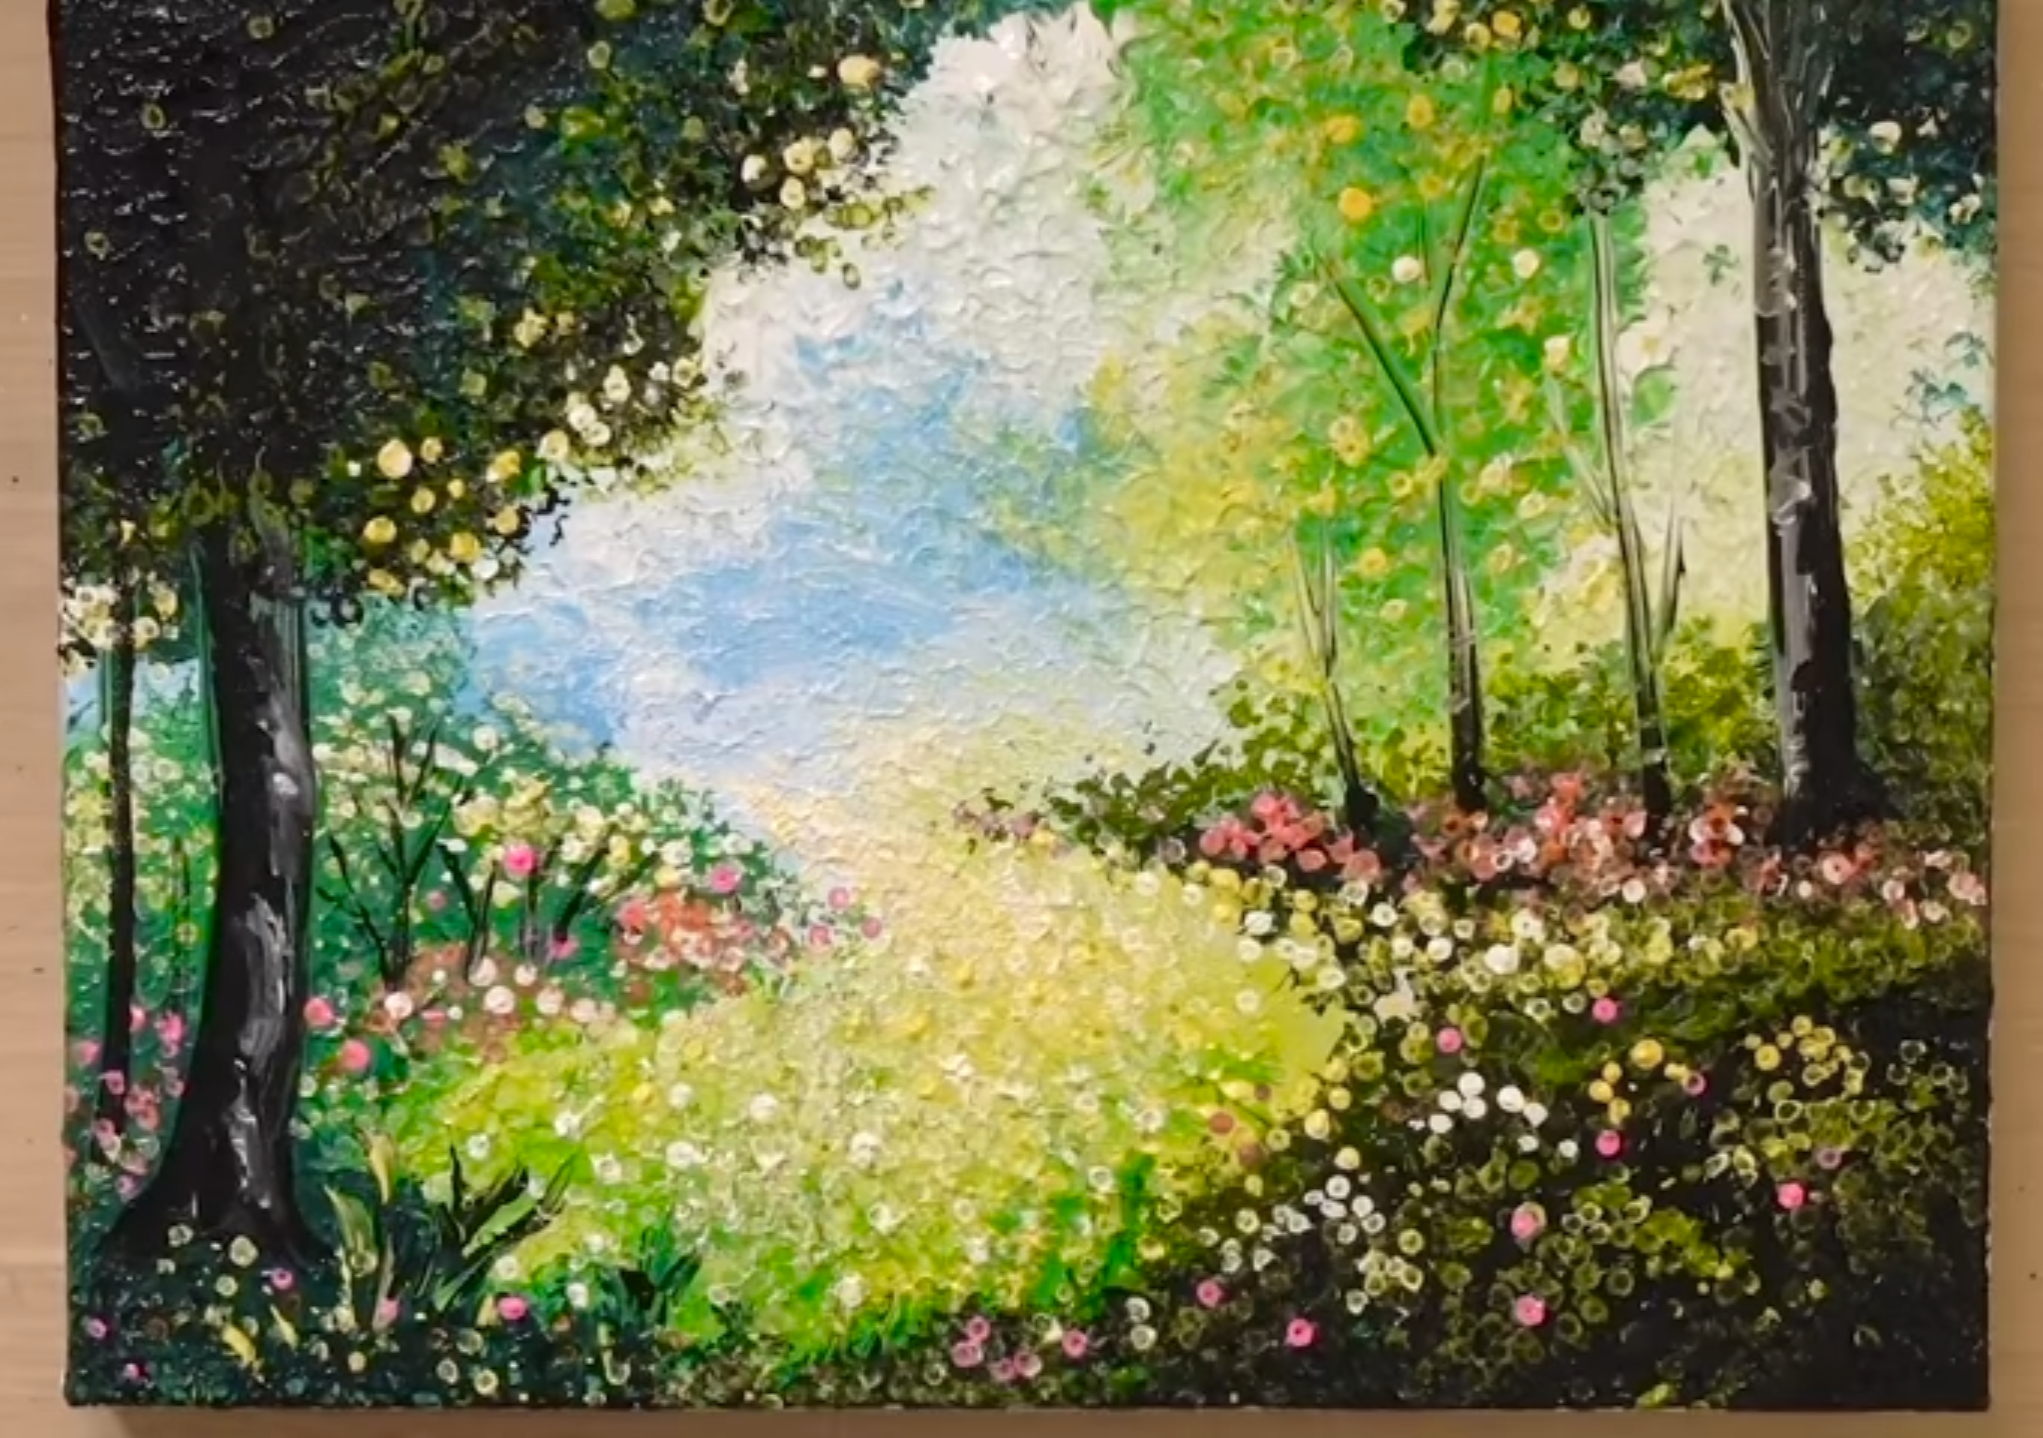
\includegraphics[width=0.24\textwidth]{painting_example_layer_2.png}}
    \subfloat{\includegraphics[width=0.24\textwidth]{painting_example_layer_3.png}}
    \caption{ Фон | Рельеф фона | Детализация заднего плана | Основные объекты}
    \label{fig:layered_painting}
\end{figure}
\FloatBarrier


Поэтому стоит попробовать сначала заполнять картинку толстыми, грубыми мазками
(то есть просто с большей шириной, а в реальной жизни это будет отражаться в большем размере кисти и в более сильном нажатии).

\subsection{Добавить возможность использования локальных методов оптимизации}\label{subsec:local-methods}
Такие методы, как \textbf\textit{{градиентный спуск}} и \textbf\textit{{метод Ньютона}} позволяют достичь гораздо большей скорости сходимости
(в случае метода ньютона — сходимость квадратичная (\url{http://w.ict.nsc.ru/books/textbooks/akhmerov/mo_unicode/4.html})),
но требуют умения посчитать градиент функции ошибки в любой точке, а также вектор вторых производных по каждому из аргументов.

Сами алгоритмы реализованы и находятся в этой папке: \url{https://github.com/donRumata03/PowerfulGA/blob/master/other_optimization/}.
Предусмотрена опция подсчёта первой и вторых производных через подстановку близких значений параметров:

\begin{equation}
    f'(x_0) \approx \frac{f(x_0 + \Delta x) - f(x_0)}{\Delta x}
\end{equation}

Однако в случае с мазками при маленьких изменениях параметров функция ошибки остаётся неизменной, так как это приводит к такому же набору закрашенных пикселей.
Соответственно, нужно либо радикально увеличивать разрешение изображения, либо использовать аналитические методы.
То есть нужно математически посчитать изменение функции ошибки при бесконечно малом изменении из параметров функции.

\subsection{Организовать систему тестирования различных алгоритмов на различных функциях}\label{itm:testing_system}
Звучит как нечто весьма простое, но реальность сложнее, чем кажется.
Напрашивающийся вариант — дать каждому алгоритму заданное количество вычислений функции ошибки и сравнить, какой результат они получат.

Однако функция ошибки нелинейная, поэтому сложно будет понять,
насколько сильному различию в качестве алгоритма соответствует полученная численная разница в результатах.

Целесообразно сравнивать количество итераций, требующееся алгоритмам для получения заданного результата.
Но и тут не всё так просто: нельзя просто запустить алгоритмы на неограниченное количество итераций
и ждать достижения нужного значения функции,
так как во многих из них (как минимум — в моей модификации ГА) то,
как будет проведена каждая отдельная итерация, сильно зависит от процента выполнения на момент её прохождения:
происходит планирование,  использующее информацию о максимальном количестве итераций.

Поэтому нет никакого другого выхода, кроме того, чтобы запускать этот алгоритм с разным количеством итераций и смотреть, когда он в среднем будет доходить до заданного порога.
Это необходимо автоматизировать.

В идеальном случае для поиска порога можно было бы использовать бинарный поиск, но в реальности (с поправкой на шум) имеет смысл использовать эвристическую модификацию н-арного поиска (объяснить!).
Для полной оценки планируется построить график достаточного количества итераций от требуемого значения функции в интересующей нас зоне.

Это нужно проделать для нескольких сложных функций (например, из списка в Википедии \href{https://en.wikipedia.org/wiki/Test_functions_for_optimization}{https://en.wikipedia.org/wiki/Test_functions_for_optimization})
и на основе этого сделать вывод об общем качестве работы.

Умение хорошо оценивать работу алгоритма «в полной комплектации» даёт возможность оптимизировать гиперпараметры.
То есть мы запускаем мета-алгоритм, параметры которого — это гиперпараметры основного алгоритма, а функция ошибки — качество его работы.
В случае с ГА, например, гиперпараметрами могут быть: hazing\_percent, elite или hyperelite \_fit\_pow, epoch\_pow, mutation\_percent\_sigma, target\_gene\_mutation\_number и т.д.


\subsection{Контроль уровня разнообразия особей в ГА}\label{subsec:control_GA_diversity}
Известно (\ref{subsubsec:hazing}), что в ГА важен баланс между скоростью сходимости и разнообразием в популяции.
Второе важно, чтобы преждевременно не попасть в локальный оптимум, а получше «исследовать» всю часть пространства, отведённую для поиска.

Есть много механизмов для изменения баланса (они также описаны в \ref{subsubsec:hazing}).
Однако сейчас эти механизмы действуют вслепую — по заранее заготовленному плану, не зависящему от текущей ситуации в популяции.
Нужно перейти от задания действий перед запуском программы к заданию требуемых результатов.
А именно — нужно:
\begin{enumerate}
    \item Задать метрику разнообразия, устойчивую к помехам и выдающую данные в человекочитаемом формате (чтобы задавать её зависимость).
    \item Научиться использовать регуляторные средства ( \ref{subsubsec:hazing}) для перевода популяции к заданному значению метрики.
    \item На основе экспериментов определить, какой должна быть зависимость требуемого значения метрики от процента выполнения.
\end{enumerate}

\subsubsection{Задание метрики}
Важно, что она должна быть сравнима при подсчёте для разных функций и областей, жалательно — находясь всё время в том же интервале, например,
$\in [0; 1]$.

В простом случае можно считать метрику как отношение n-мерного «объёма» выпуклой оболочки к n-мерному «объёму» всего пространства поиска.
(алгоритм нахождения МВО в n-мерном пространстве: \url{https://neerc.ifmo.ru/wiki/index.php?title=%D0%92%D1%8B%D0%BF%D1%83%D0%BA%D0%BB%D0%B0%D1%8F_%D0%BE%D0%B1%D0%BE%D0%BB%D0%BE%D1%87%D0%BA%D0%B0_%D0%B2_n-%D0%BC%D0%B5%D1%80%D0%BD%D0%BE%D0%BC_%D0%BF%D1%80%D0%BE%D1%81%D1%82%D1%80%D0%B0%D0%BD%D1%81%D1%82%D0%B2%D0%B5})

Проблемой этой метрики может стать то, что в пространствах с высокой и низкой  размерностью при таком же количестве точек могут быть несопоставимые результаты.

Однако понятно, что может быть несколько точек «по краям», а все остальные — сконцентрированы на одном пятачке.
Метрика покажет, что точки достаточно диверсифицированы, что окажется неверным.

Варианты исправить этот недочёт такие:
либо как-то отбросить сколько-то процентов самых «дальних» точек (ӹӝ «выбросы») или пытаться выделять «очаги» — скопления точек,
либо производить те же операции учитывая все точки, но «нечётко»: например, вместо того, чтобы не учитывать точку, учитывать её с маленьким весом.

Проще всего — удалять каждый раз точку, максимально удалённую от «центра масс» (постоянно поддерживая актуальное его местоположение),
убрав таким образом $\approx 10\%$ точек, а потом найти отношение объёмов.

Другой напрашивающийся подход — сначала посчитать в сетке точек (например, $\approx 10$ по каждому измерению)
значение плотности распределения геномов вокруг этой точки, потом для каждого генома определить, в зоне с какой примерной плотностью он находится и, например, просуммировать эти значения,
потом сравнить результат со значением для идеально равномерного распределения и для всех геномов, находящихся в одной точке и откалибровать, переведя в шкалу от 0 до 1.

Однако для пространств с высокой размерностью высокой размерностью (то есть с большим количеством параметров) такое произвести не получится, так как количество узлов
для достаточной детализации становится слишком большим:
\begin{equation}
    N_{nodes} = segments\_per\_axis^{dimensions}
\end{equation}
То есть для 10-и делений по оси уже для 9-и параметров оказывается совершенно неприемлемое число операций.

Но в таком случае можно считать плотность не в узлах, которых становится больше, чем точек.

% TODO Сказать про большие размерности: плотность не посчитать, концентрация мала
% TODO  кластеризация, K-means?
% TODO  на практике лучше отдельно по осям и по их комбинациям, так как мало скоррелировано, то есть маловероятно, что по всем осям будет равномерное распреледение, а в ком=мбинации — нет хотя такое возможно


\subsection{Улучшить алгоритм поиска цветов и разделения на зоны}\label{subsec:posterisation_and_zoning}

Сейчас для разделения изображения на зоны используется Adobe Illustrator.
По заданному количеству цветов (и, следовательно, уровню детализации) он разделяет изображение на зоны,
присваивая каждой какой-то из цветов палитры так, чтобы он хорошо .
Сама палитра тоже формируется в ходе работы алгоритма.

Скорее всего, для этого используется один из популярных алгоритмов, описанных \href{https://en.wikipedia.org/wiki/Color_quantization}{здесь}, или некая проприетарная их вариация.
Зоны, на которые происходит деление, описываются частями плоскости, ограниченными кривыми безье — «path»  формате $svg$.

Несмотря на то что формально алгоритм выполняет свою работу, большое количество зон имеет очень продолговатую форму,
а также наблюдается неимоверный разброс в размерах между разными зонами (см. \ref{subsec:inequality}):
всё это уменьшает эффективность процесса.

% TODO: написать про свой алгоритм и склеивание зон

\subsection{Перенести графические вычисления на видеокарту}\label{subsec:move_graphics_to_videocard}
Также напрашивающееся улучшение.
Это может существенно ускорить работу алгоритма, особенно — генетического (так как при нём можно распараллелить вычисление для целой популяции),
причём только в случае, если не используется быстрый пересчёт функции ошибки или мутирует очень много мазков одновременно.
Как бы то ни было, когда-нибудь стоит добавить эту возможность.
Тестовый проект с использованием OpenCL я уже написал.

Изначальная картинка будет переноситься в видеопамять один раз — в начале работы программы.
Выделить память для матрицы можно также один раз, а потом каждый раз её очищать (эту операцию можно производить параллельно).

Если использовать видеокарту для распараллеливания вычислений, встаёт вопрос, на каком именно уровне производить разделение.
Варианты такие:
\begin{enumerate}
    \item Каждое изображение — на своём потоке.
    Такой способ подходит только для ГА в случае огромного размера поколения (так как потоков у видеокарты порядка нескольких тысяч).
    Для отжига — никогда.

    \item Каждый мазок — на своём потоке.
                Тут возникают проблемы с синхронизацией, так как порядок наложения важен: как минимум не должны появляться в хаотическом порядке пиксели из мазков разного цвета.
                Даже если происходит смешение цветов при наложении, синхронизация важна.
                Это можно сделать через дополнительную струкрутру данных в виде прямоугольной матрицы, в которой для каждого пикселя будет записываться список цветов с приоритетами
                (индексами мазков, а значит, и числами, определяющими порядок слоёв).
                Потом уже независимо для каждого пикселя будет происходить обработка смешения или наложения с замещением «попавших» на него цветов.
                Всё упирается в умение синхронизировать потоки.
                Тут нужно либо симуляцию мьютекса для каждого пикселя (то есть матрицу булевых значений «занят-не занят»),
                либо умение распределить мазки по потокам так, чтобы в каждый момент времени не было никаких двух с накладывающимися bounding-box'ами.

                В первом случае либо нужно покупать видеокарту с поддержкой атомарных значений, либо придётся вставлять дополнительные проверки,
                чтобы два потока не прочитали почти одновременно состояние «не занят»  и не зашли туда до того, как какой-либо из них успеет записать состояние «закрыто».

                Во втором случае уменьшится количество потоков, одновременно работающих над одной «картиной».


    \item Проводить распараллеливыание на графическом примитиве нисшего уровня, использующемся в данном алгоритме (см. \ref{subsec:rasterization}).
                Например, полигоны или круги.
                Видеокарта умеет эффективно отрисовывать такие примитивы.
                Однако количество точек в примитивах обычно невелико: существенно меньше, чем ядер в видеокарте.
\end{enumerate}
Причём всегда можно комбинировать разделения на разных уровнях.

Когда будет произведена растеризация, на той же видеокарте посчитается функция ошибки: в этом случае легко сделать это независимо для каждого пикселя.
Единственное — нужно помнить, что для добавления наказания за наложения и пустоты в функцию ошибки надо составлять дополнительные матрицы, в которых это будет указано.


Адаптация алгоритмов под видеокарту описана здесь: \ref{subsec:rasterization}.

\subsection{Выделение границ мазками}
Ни для кого не секрет, что существует много алгоритмов, позволяющих с неплохой точностью выделять «границы» у изображения —
резкие цветовые (а иногда и содержательные, основанные на границах распозненных объектов или их паттернов!) переходы.
Предположительно, их использование могло бы повысить качество работы алгоритма: дополнительная проработка границ увеличит чёткость
и «читаемость» картины.
Остаётся вопрос — как расположить точки, задающие мазки, чтобы робот обвёл границы объектов.
Конечно же, будет применяться оптимизация, а «нарезать» линии границ можно, например, по их резким поворотам.
